\documentclass[a4paper,12pt]{article}
\usepackage{array}
\usepackage{graphicx}
\graphicspath{ {images/} }
\usepackage{geometry}
 \geometry{
 a4paper,
 left=20mm,
 top=20mm,
 right=20mm
 }
 \begin{document}
\centering{\textsf{\huge{Ankit Gala}}}
\noindent\makebox[\linewidth]{\rule{170mm}{0.4pt}}
\begin{flushleft}
{B-208,\hfill{Contact : 7208760344} \\ Saryu Apartments,\hfill{Email ID: ankitg444@gmail.com}\\Ashok nagar\\Kandivali(east) \\Mumbai-400101.}
\end{flushleft}
\hfill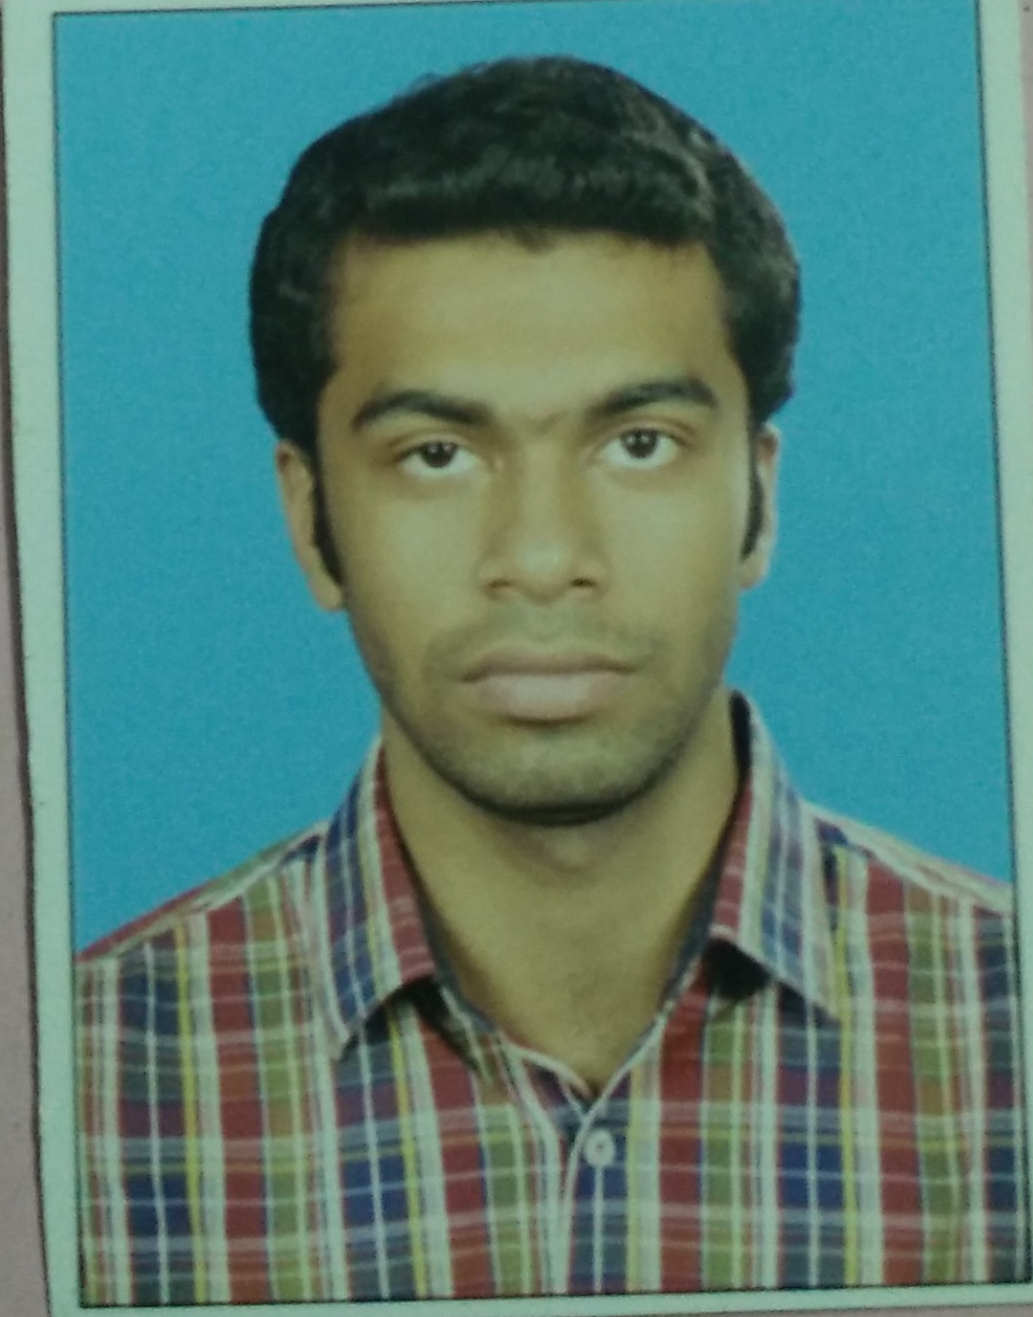
\includegraphics[width=20mm,height=20mm]{Untitled}\\[1cm]
\begin{flushleft}

\underline{\textbf{OBJECTIVE}}:\\
To excel in my field through hard work, research, skills and perseverance.To live honest and hard life to work in a highly challenging competitive environment for the enhancement of my creative abilities.\\[0.5cm]

\underline{\textbf{EDUCATION}}:\\[0.5cm]
\begin{tabular}{ | m{2.5cm} | m{3cm}| m{2.5cm} | m{2.5cm}| m{3cm} | } 
\hline
Degree& College/School & University & Passing Year & Passing Percentage \\ 
\hline
10th & Children's Academy & Maharashtra Board & 2012 & 93.63 \\ 
\hline
12th & T.P.Bhatia college & Maharashtra Board & 2014 &84.31 \\ 
\hline
B.Tech & V.J.T.I,Mumbai & Mumbai University &2018 & 8.75(till 3rd semester) \\
\hline
\end{tabular}\\[0.5cm]
\underline{\textbf{PROJECTS}}:\\[0.5cm]
\begin{enumerate}
    \item {Website Development Project }
    \item{Suduko solver(Java)}
\end{enumerate}
\underline{\textbf{TRAINING \& INTERNSHIP}}:\\[0.5cm]
\begin{itemize}
 \item{e-YANTRA Summer Internship-2016}
\end{itemize}
\underline{\textbf{RESEARCH PUBLICATIONS}}:\\[0.5cm]
\underline{\textbf{TECHNICAL SKILLS}}:\\[0.5cm]
Programming languages and technology:

\begin{itemize}
 \item{C,C++,Embedded C}
 \item{Java}
 \item{HTML,CSS,Bootstrap}
 \item{Javascript,Jquery}
 \item{Php,SQL}
 \item{Python}
\end{itemize}
\underline{\textbf{SOFT SKILLS}}:\\[0.5cm]
\begin{enumerate}
 \item{Problem Solving}
 \item{Time management}
 \item{Team work}
\end{enumerate}
\underline{\textbf{EXTRA-CURRICULAR ACTIVITIES }}:\\[0.5cm]
\begin{itemize}
 \item{Sports}
 \item{Travelling}
\end{itemize}
\underline{\textbf{CO-CURRICULAR ACTIVITIES }}:\\[0.5cm]
\begin{enumerate}
 \item{Participating in coding competitions}
 \item{Robotics}
\end{enumerate}
\underline{\textbf{PERSONAL DETAILS }}:\\[0.5cm]
Father's name:Pankaj Gala\\
Mother's name:Mita Gala\\
Sex:Male\\
Date of Birth:February 24,1996\\
Nationality:Indian\\
Marital Status:Single\\[0.5cm]


 \end{flushleft}

\end{document}
